\documentclass[a4paper,12pt]{extarticle}

\usepackage[utf8x]{inputenc}
\usepackage[T1,T2A]{fontenc}
\usepackage[russian]{babel}
\usepackage{hyperref}
\usepackage{indentfirst}
\usepackage{listings}
\usepackage{color}
\usepackage{here}
\usepackage{array}
\usepackage{multirow}
\usepackage{graphicx}
\usepackage{caption}
\usepackage{subcaption}
\usepackage{chngcntr}
\usepackage{amsmath}
\usepackage{amssymb}
\usepackage{pgfplots}
\usepackage{pgfplotstable}
\renewcommand{\lstlistingname}{Программа} % заголовок листингов кода

\bibliographystyle{ugost2008ls}

\usepackage{listings}
\lstset{ %
extendedchars=\true,
keepspaces=true,
language=C++,						% choose the language of the code
basicstyle=\scriptsize,		% the size of the fonts that are used for the code
numbers=left,					% where to put the line-numbers
numberstyle=\scriptsize,		% the size of the fonts that are used for the line-numbers
stepnumber=1,					% the step between two line-numbers. If it is 1 each line will be numbered
numbersep=5pt,					% how far the line-numbers are from the code
backgroundcolor=\color{white},	% choose the background color. You must add \usepackage{color}
showspaces=false				% show spaces adding particular underscores
showstringspaces=false,			% underline spaces within strings
showtabs=false,					% show tabs within strings adding particular underscores
frame=single,           		% adds a frame around the code
tabsize=2,						% sets default tabsize to 2 spaces
captionpos=t,					% sets the caption-position to top
breaklines=true,				% sets automatic line breaking
breakatwhitespace=false,		% sets if automatic breaks should only happen at whitespace
escapeinside={\%*}{*)},			% if you want to add a comment within your code
postbreak=\raisebox{0ex}[0ex][0ex]{\ensuremath{\color{red}\hookrightarrow\space}},
texcl=true,
inputpath=fig,                     % директория с листингами
}

\usepackage[left=2cm,right=2cm,
top=2cm,bottom=2cm,bindingoffset=0cm]{geometry}

%% Нумерация картинок по секциям
\usepackage{chngcntr}
\counterwithin{figure}{section}
\counterwithin{table}{section}

%%Точки нумерации заголовков
\usepackage{titlesec}
\titlelabel{\thetitle.\quad}
\usepackage[dotinlabels]{titletoc}

%% Оформления подписи рисунка
\addto\captionsrussian{\renewcommand{\figurename}{Рисунок}}
\captionsetup[figure]{labelsep = period}

%% Подпись таблицы
\DeclareCaptionFormat{hfillstart}{\hfill#1#2#3\par}
\captionsetup[table]{format=hfillstart,labelsep=newline,justification=centering,skip=-10pt,textfont=bf}

%% Путь к каталогу с рисунками
\graphicspath{{fig/}}


\begin{document}	% начало документа

% Титульная страница
\begin{titlepage}	% начало титульной страницы

	\begin{center}		% выравнивание по центру

		\large Санкт-Петербургский Политехнический Университет Петра Великого\\
		\large Институт компьютерных наук и технологий \\
		\large Кафедра компьютерных систем и программных технологий\\[6cm]
		% название института, затем отступ 6см
		
		\huge Вычислительная математика\\[0.5cm] % название работы, затем отступ 0,5см
		\large Отчет по лабораторной работе №1\\[0.1cm]
		\large <<Сравнение точности интерполяционных полиномов>>\\[0.1cm]
		\large Вариант №5\\[5cm]

	\end{center}


	\begin{flushright} % выравнивание по правому краю
		\begin{minipage}{0.25\textwidth} % врезка в половину ширины текста
			\begin{flushleft} % выровнять её содержимое по левому краю

				\large\textbf{Работу выполнил:}\\
				\large Ламтев А.Ю.\\
				\large {Группа:} 23501/4\\
				
				\large \textbf{Преподаватель:}\\
				\large Цыган В.Н.

			\end{flushleft}
		\end{minipage}
	\end{flushright}
	
	\vfill % заполнить всё доступное ниже пространство

	\begin{center}
	\large Санкт-Петербург\\
	\large \the\year % вывести дату
	\end{center} % закончить выравнивание по центру

\thispagestyle{empty} % не нумеровать страницу
\end{titlepage} % конец титульной страницы

\vfill % заполнить всё доступное ниже пространство


\section{Цель работы}
Численно решить дифференциальное уравнение 2-го порядка.

\section{Решаемые задачи}
\begin{enumerate}

\item Привести дифференциальное уравнение второго порядка

\label{equation:1}
\begin{equation}
	t(t+1)y'' + (3t+2)y'  + y = 0
\end{equation}

к системе двух дифференциальных уравнений первого порядка.

	Начальные условия: $\left.y \right|_{t=1} = 1$, $\left.y' \right|_{t=1} = -1$, $t \in[1, 2]$  

    Точное решение: $y(t)=\frac{1}{t}$	

\item Решить с шагом $h = 0.1$

\begin{enumerate}[label=\arabic*)]
\item Используя RKF45
\item Используя метод Эйлера-Коши
\end{enumerate}

\item Сравнить результаты полученные двумя методами с точным решением.

\end{enumerate}

\section{Ход выполнения работы}

Вначале дифференциальное уравнение \ref{equation:1} засчёт подстановок $x_1(t) = y(t)$ и $x_2(t) = y'(t)$ было приведено к системе:

%\begin{displaymath}
%\begin{cases}
%	x'_1(t) = 0 \cdot x_1(t) + 1 \cdot x_2(t)
%	\\
%	x'_2(t) = - \frac{1}{t(t+1)} \cdot x_1(t) - \frac{3t+2}{t(t+1)} \cdot x_2(t)
%\end{cases}
%\end{displaymath}

\begin{displaymath}
\begin{pmatrix}
    x'_1(t) \\
    x'_2(t) \\
\end{pmatrix}
  =
\begin{pmatrix}
    0 & 1 \\
    - \frac{1}{t(t+1)} & -\frac{3t+2}{t(t+1)} \\
\end{pmatrix}
\cdot
\begin{pmatrix}
    x_1(t) \\
    x_2(t) \\
\end{pmatrix}
\end{displaymath}

Затем было разработано программное обеспечение на языке программирования \textbf{java}, позволяющее решить поставленные задачи. Данное программное обеспечение включает в себя:
\begin{itemize}

\item Библиотеку \textbf{Diffeqs}.

 Она включает в себя функцию \textbf{rkf45}, которая содержит вызов стандартной форсайтовской функции \textbf{rkf45}, разработанной на языке программирования \textbf{с}.

 Еще \textbf{Diffeqs} содержит самостоятельно написанную функцию \textbf{eulerCauchy}. Данная функция численно решает дифференциальные уравнения, используя метод Эйлера-Коши 2-й степени.
 
\begin{displaymath}
\begin{cases}
	x_{n+1}^{*} = x_n + hf(t_n, x_n)
	\\
	x_{n+1} = x_n + \frac{h}{2} \Big (f(t_n, x_n) + f(t_{n+1}, x_{n+1}^{*}) \Big) 
\end{cases}
\end{displaymath} 
 
 Функция \textbf{eulerCauchy} представлена в листинге \ref{code:EulerCauchy}.

\item Приложение, решающее заданную систему дифференциальных уравнений точно (по формуле $y(t) = \frac{1}{t}$), при помощи \textbf{rkf45} и функцией \textbf{eulerCauchy}, реализующей метод Эйлера-Коши (листинг \ref{code:Lab3}).

\end{itemize}

На рисунках \ref{pic:demo1} - \ref{pic:demo3} изображен вывод работы программы: результат решения системы дифференциальных уравнений на отрезке $[1, 2]$ с шагом $h=0.1$ стандартной функцией \textbf{rkf45} с установленной относительной погрешностью $10^{-13}$, функцией \textbf{eulerCauchy} и по аналитически полученной точной формуле соответственно.

\begin{figure}[H]
    \centering
    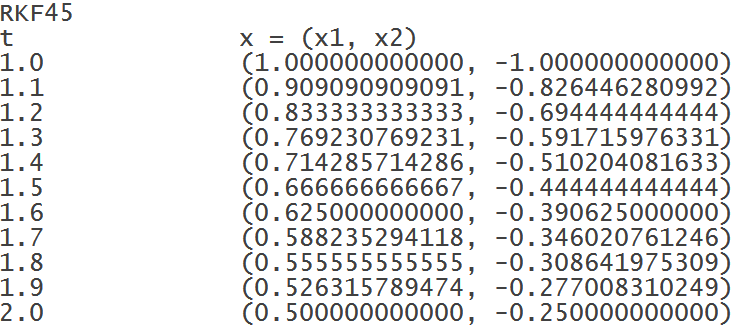
\includegraphics[height=2.2in]{rkf45}
    \caption{Вывод программы: RKF45}
    \label{pic:demo1}
\end{figure} 

\begin{figure}[H]
    \centering
    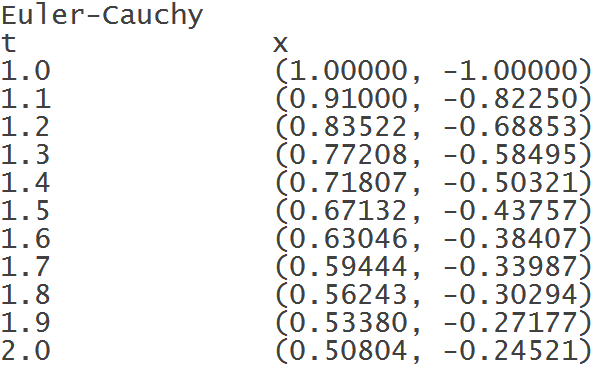
\includegraphics[height=2.2in]{euler_cauchy}
    \caption{Вывод программы: метод Эйлера-Коши}
    \label{pic:demo2}
\end{figure} 

\begin{figure}[H]
    \centering
    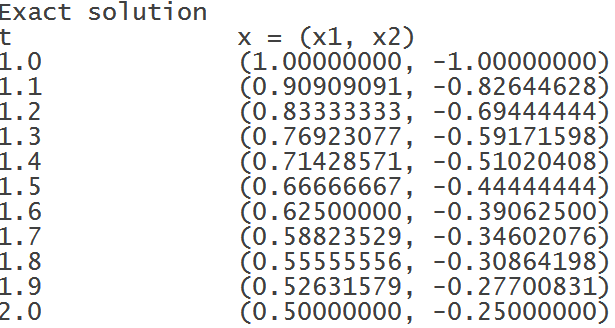
\includegraphics[height=2.2in]{exact}
    \caption{Вывод программы: точное решение}
    \label{pic:demo3}
\end{figure} 

По выводу программы видно, что значения, полученные с использованием функции \textbf{rkf45}, совпадают с точными значениями с точностью 12 знаков после точки, а значения, полученные методом Эйлера-Коши имеют точность 1 - 2 знака после точки. 

На рисунке \ref{pic:graphic1} изображены графики точного решения исходного дифференциального уравнения \ref{equation:1} и решения методом Эйлера-Коши:

\begin{figure}[H]
\begin{center}
	\begin{tikzpicture} [every plot/.append style={thick}]
		\begin{axis}[			
			height=0.5\textheight,
			width=1.0\textwidth,
			legend pos=north east,
			xlabel={$t$},
			ylabel={$y(t)$},
			xlabel near ticks,
			ylabel near ticks,			
			xmax=2.0,
			xmin=1.0,
			ymax=1.0,
			ymin=0.5,
			xmode=linear,			
			grid=major
		]
		\addplot table[x=t,y=exactValue,col sep=comma]{data/exactValues.csv};
		%\addplot table[x=t,y=rkf45Value,col sep=comma]{data/rkf45Values.csv};
		\addplot table[x=t,y=eulerCauchyValue,col sep=comma]{data/eulerCauchyValues.csv};
		\legend{Точное решение: $\frac{1}{t}$, Метод Эйлера-Коши}
		\end{axis}
	\end{tikzpicture}
	\caption{График точного решения и решения методом Эйлера-Коши}
	\label{pic:graphic1}
\end{center}
\end{figure}

По графику на рисунке \ref{pic:graphic2} видно, что чем ближе к концу отрезка $[1, 2]$, тем сильнее решение методом Эйлера-Коши отклоняется от точного решения.

Построим график погрешности решения метом Эйлера-Коши на отрезке $[1, 2]$:

\begin{figure}[H]
\begin{center}
	\begin{tikzpicture} [every plot/.append style={thick}]
		\begin{axis}[			
			height=0.25\textheight,
			width=1.0\textwidth,
			xlabel={$t$},
			ylabel={$|\varepsilon(t)|$},
			xlabel near ticks,
			ylabel near ticks,			
			xmax=2.0,
			xmin=1.0,
			ymax=0.0081,
			ymin=0.0,
			%ymode=log,
			%log basis y=10, 
			grid=major
		]
		\addplot table[x=t,y=eulerCauchyEpsilon,col sep=comma]{data/eulerCauchyEpsilons.csv};
		\end{axis}
	\end{tikzpicture}
	\caption{Погрешность решения методом Эйлера-Коши на каждом шаге на $[1, 2]$}
	\label{pic:graphic2}
\end{center}
\end{figure}

Локальная погрешность монотонно возрастает на отрезке $[1, 2]$ , принимая значения от 0 до $8 \cdot 10^{-3}$. Определим, является ли это нормой.

Для метода 2-й степени формула приближения главного члена погрешности имеет вид: 
\begin{displaymath}
\varepsilon_{n+1} = \frac{h^3 \cdot x'''(\eta)}{3!}\text{, где $\eta \in a\dots b$}
\end{displaymath}

Вычислим приближенное значение локальной погрешности метода Эйлера-Коши на первом шаге:

\begin{displaymath}
\varepsilon_{1} = \frac{h^3 \cdot x'''(\eta)}{3!} = \left.\frac{h^3 \cdot \frac{-6}{t^4}}{6} \right|_{t=\eta} = \left.-\frac{h^3}{t^4} \right|_{t=\eta} = -\frac{{0.1}^3}{1^4} = -10^{-3}
\end{displaymath}

Получили, что значения реальной локальной погрешности на отрезке $[1, 2]$ пропорциональны значению теоретической локальной погрешности на первом шаге и превышают значение теоретической локальной погрешности (начиная с третьего шага) меньше, чем на порядок. Превышение объясняется накоплением глобальной погрешности.

\section{Выводы}

Решение системы дифференциальных уравнений при помощи функции \textbf{rkf45} оказалось более точным, чем решение методом Эйлера-Коши. Полученный результат был ожидаем, потому что функция \textbf{rkf45} реализует методы Рунге-Кутты 4-й и 5-й степени, в то время как метод Эйлера-Коши имеет лишь 2-ую степень. Точность, полученная при решении системы дифференциальных уравнений методом Эйлера-Коши оказалась сопоставимой с точностью метода 2-й степени и поэтому функция \textbf{eulerCauchy} скорее всего составлена верно.

\newpage

\section*{Приложение 1. Листинги кода}

\captionof{lstlisting}{Приложение}
\lstinputlisting[label=code:Lab3, linerange={1-162}]{../../../app/src/main/java/com/lamtev/comp_maths_labs/lab3/app/Lab3.java}
\parindent=1cm

\captionof{lstlisting}{Функция eulerCauchy}
\lstinputlisting[label=code:EulerCauchy, linerange={1-41}]{../../../diffeqs_lib/src/main/java/com/lamtev/comp_maths_labs/lab3/diffeqs_lib/EulerCauchy.java}
\parindent=1cm

\end{document}
